% !Mode:: "TeX:UTF-8"
% VL 11, gebaut aus part-architekturen-anwendungen/20-faltung-cnn.md
% (Dialogmuster und Zeiten: transcripts/vl10-faltung-cnn-2025/notiz.md).
% !Mode:: "TeX:UTF-8"
\newcommand{\thepage}{} % to silence a hyperref warning about pdfpagelabels
\RequirePackage[]{silence}
\WarningsOff[hyperref]
\PassOptionsToPackage{log-declarations=false}{xparse}
%\RequirePackage[l2tabu, orthodox]{nag}
\RequirePackage{luatex85} % to make \pdf...= commands work with LuaTeX
\documentclass[aspectratio=169,t]{beamer}
\usepackage{ifthen}
\usepackage[T1]{fontenc}
\usepackage{iftex}
\ifLuaTeX
 \usepackage{fontspec}
 \setmainfont[Ligatures=TeX]{Source Sans Pro}
\else
 \usepackage[utf8]{inputenc}
\fi
\usepackage{german}
\usepackage{newunicodechar}
\newunicodechar{€}{\texteuro}
\newunicodechar{ß}{\ss}
\renewcommand{\SS}{\iffontchar\font"1E9E \symbol{"1E9E}\else SS\fi}
\usepackage{ellipsis}
\usepackage{microtype}
\usepackage{listings}
\usepackage{sourcecodepro}
\lstset{language=Python, basicstyle=\ttfamily}
\usepackage{amsfonts}
\usepackage{amssymb}
\usepackage{amsthm}
\usepackage{fancyhdr}
\usepackage{graphicx}

\newtheorem{proposition}[theorem]{Proposition}

\DeclareMathOperator*{\argmax}{argmax}
\DeclareMathOperator{\supp}{supp}
\newcommand{\E}{\ensuremath{\mathbb{E}}}
\newcommand{\V}{\ensuremath{\mathbb{V}}}

\setbeamercolor{emph}{fg=purple}
\renewcommand<>{\emph}[1]{%
  {\usebeamercolor[fg]{emph}\only#2{\itshape}#1}%
}



\hypersetup{draft=false,colorlinks=false,pdfpagemode=UseOutlines,plainpages=false,
            breaklinks=true,bookmarksnumbered=true,pdfborder=0 0 0,
            pdftitle={Einführung in Deep Learning WiSe 2026/27 HHU},
            pdfauthor={Konrad Voelkel},
            pdfsubject={data science}}

%\documentclass[aspectratio=169,t]{beamer}
\usetheme{hhubeamer} % put the hhu-beamer-theme in /usr/share/texmf/tex/latex/beamer/themes/

% -------------------- Code listings config --------------------
% Define custom colors for syntax highlighting
\definecolor{codegreen}{rgb}{0,0.6,0}
\definecolor{codegray}{rgb}{0.5,0.5,0.5}
\definecolor{codepurple}{rgb}{0.58,0,0.82}
\definecolor{backcolour}{rgb}{0.96,0.96,0.94} % Very light gray/beige
% Configure the listings package
\lstset{
    language=Python,
    backgroundcolor=\color{backcolour},   
    commentstyle=\color{codegreen}\itshape,
    keywordstyle=\color{blue}\bfseries,
    numberstyle=\tiny\color{codegray},
    stringstyle=\color{codepurple},
    basicstyle=\ttfamily\footnotesize, % Use a monospaced font
    breakatwhitespace=false,         
    breaklines=true,      
             % Enable automatic line breaking
    captionpos=b,                      % Caption at the bottom
    keepspaces=true,                 
    numbers=left,                      % Line numbers on the left
    numbersep=10pt,                    % Distance of line numbers from the code
    showspaces=false,                
    showstringspaces=false,            % Don't show weird underscores in strings
    showtabs=false,                  
    tabsize=4,
    frame=single,                      % Add a subtle border around the code
    rulecolor=\color{black!20},        % Border color
  }

\event[]{}
\author[Wintersemester 2026/27]{Dr. Konrad Völkel, Wintersemester 2026/27}

%\title{Data Science, VL 1}
%\date{16.04.2026}


%%% Local Variables:
%%% mode: latex
%%% TeX-master: t
%%% End:


% Fassung mit Dozentennotizen (zweiter Schirm): die nächste Zeile einkommentieren.
% \setbeameroption{show notes on second screen=right}

\graphicspath{{../images/}}

\title[Faltung und CNNs (VL 11)]{Faltung und CNNs\\\large Einführung in Deep Learning, VL 11}
\date{06.01.2027}

\begin{document}

\begin{frame}
  \titlepage

  \note{\textbf{Ablauf, 90 Minuten} (2025: 41 Min. Folien, 20 Min. Browser, 26 Min.
    Notebook):\\[2pt]
    \begin{tabular}{@{}rll@{}}
      0--6   & Folie 2       & Willkommen zurück, Übungsblatt läuft noch\\
      6--16  & Folien 3--4   & Weichzeichnen und Kanten, Hubel \& Wiesel\\
      16--28 & Folien 5--7   & 1D-Faltung: Definition, Flippen, Parameter Sharing\\
      28--38 & Folie 8       & ASML-Beispiel mit vier Filtern\\
      38--46 & Folien 9--10  & Pooling\\
      46--56 & Folien 11--12 & 2D-Faltung, GIMP-Faltungsmatrix\\
      56--68 & Folien 13--14 & Kanäle, CNN-Architektur, Ausgabegrößen\\
      68--85 & Folie 15      & \textbf{Notebook: Faltung live}\\
      85--90 & Folie 16      & Ausblick\\
    \end{tabular}\\[4pt]
    Das Notebook \texttt{VL\_10\_convolutions.ipynb} zeigen, nicht vorlesen --- 2025 hat
    es 26 Minuten gekostet. Die Live-Änderung am 2D-Filter ist der Höhepunkt.}
\end{frame}

\begin{frame}
  \frametitle{Willkommen zurück}

  \begin{center}
    \Large
    Heute: die Architektur, die 2012 alles ausgelöst hat.
  \end{center}

  \note{Das Übungsblatt aus der Zeit vor der Pause (Faltung) ist erst nächsten Mittwoch fällig;
    das nächste Blatt kommt dann heraus.
    Kurzer Rückblick: Wir haben Sequenzen gemacht, heute Bilder --- und am Ende sehen wir,
    dass beides dasselbe Prinzip ist, nur mit anderer Nachbarschaft.
    AlexNet aus VL 1 ist genau das hier.}
\end{frame}

\begin{frame}
  \frametitle{Wer weichgezeichnet hat, hat gefaltet}

  \begin{center}
    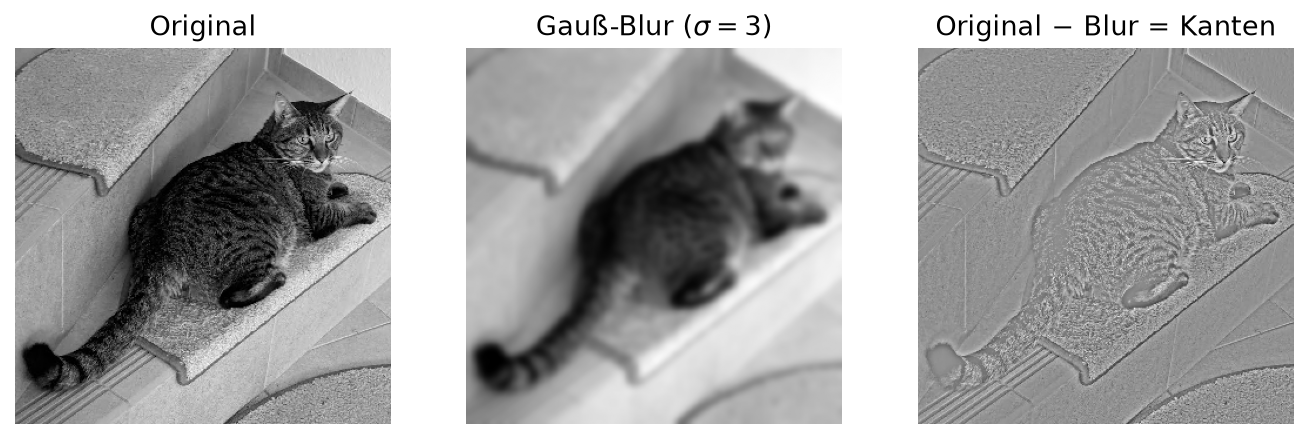
\includegraphics[width=0.78\textwidth]{vl10-blur-edges.png}
  \end{center}

  \note{Jeder Pixel wird durch einen gewichteten Mittelwert seiner Nachbarn ersetzt ---
    das ist eine Faltung. Original minus weichgezeichnet lässt genau die Kanten übrig
    („make a difference“).
    Wer GIMP oder Photoshop benutzt hat, kennt das Ergebnis, ohne den Namen zu kennen.}
\end{frame}

\begin{frame}
  \frametitle{Das Auge macht es genauso}

  \begin{center}
    \Large
    Hubel \& Wiesel (1959):\\[12pt]
    Neuronen in der Sehrinde, die nur auf Balken\\
    einer \emph{bestimmten Orientierung} antworten.
  \end{center}

  \note{Lokale Kantendetektoren --- und genau die kommen in den ersten Schichten eines
    trainierten CNN von selbst heraus. Das ist eine der schönsten Übereinstimmungen
    zwischen Biologie und Deep Learning.
    Das klassische Bild dazu steht im Wikipedia-Artikel „Orientation column“ (CC-BY-SA),
    im Skript verlinkt --- bei Bedarf im Browser zeigen.}
\end{frame}

\begin{frame}
  \frametitle{Faltung, eindimensional}

  \begin{center}
    \Huge $(f \ast g)(x) = \sum_{y=-n}^{n} f(y)\,g(x-y)$
  \end{center}

  \bigskip
  \begin{center}
    \normalsize $g$ = Signal (lang), \quad $f$ = Filter (kurz, $2n+1$ Werte)
  \end{center}

  \note{Zero padding am Rand, sonst wird das Ergebnis kürzer.
    Die Formel erstmal stehen lassen und fragen: Was steht da eigentlich?}
\end{frame}

\begin{frame}
  \frametitle{Da steht ein Skalarprodukt}

  \begin{center}
    \Large
    Ausschnitt nehmen \; $\to$ \; \emph{flippen} \; $\to$ \; Skalarprodukt
  \end{center}

  \bigskip
  \begin{center}
    \normalsize Ohne das Flippen heißt es \emph{Korrelation}.
  \end{center}

  \note{Das Flippen ist der einzige Unterschied zwischen Faltung und Korrelation, und für
    symmetrische Filter gibt es gar keinen.
    Pointe, die später wichtig wird: PyTorch lässt das Flippen weg --- und weil die Filter
    \emph{gelernt} werden, ist das völlig egal. Das Netz lernt eben den gespiegelten
    Filter.}
\end{frame}

\begin{frame}
  \frametitle{Parameter Sharing}

  \begin{center}
    \Large
    Ein Filter ist ein Neuron mit $2n+1$ Gewichten,\\
    das an \emph{jeder} Position dasselbe rechnet.
  \end{center}

  \bigskip
  \begin{center}
    \normalsize Wenige Parameter --- und Translationsäquivarianz.
  \end{center}

  \note{Zwei Konsequenzen: Die Schicht hat nur $2n+1$ Parameter, egal wie lang das Signal
    ist --- ein MLP bräuchte eine Gewichtsmatrix in Signallänge. Und: Verschiebt man das
    Signal, verschiebt sich die Antwort mit.
    Das ist der Grund, warum CNNs mit Bildern so viel besser umgehen als MLPs.}
\end{frame}

\begin{frame}
  \frametitle{Vier Filter auf einem Aktienkurs}

  \begin{center}
    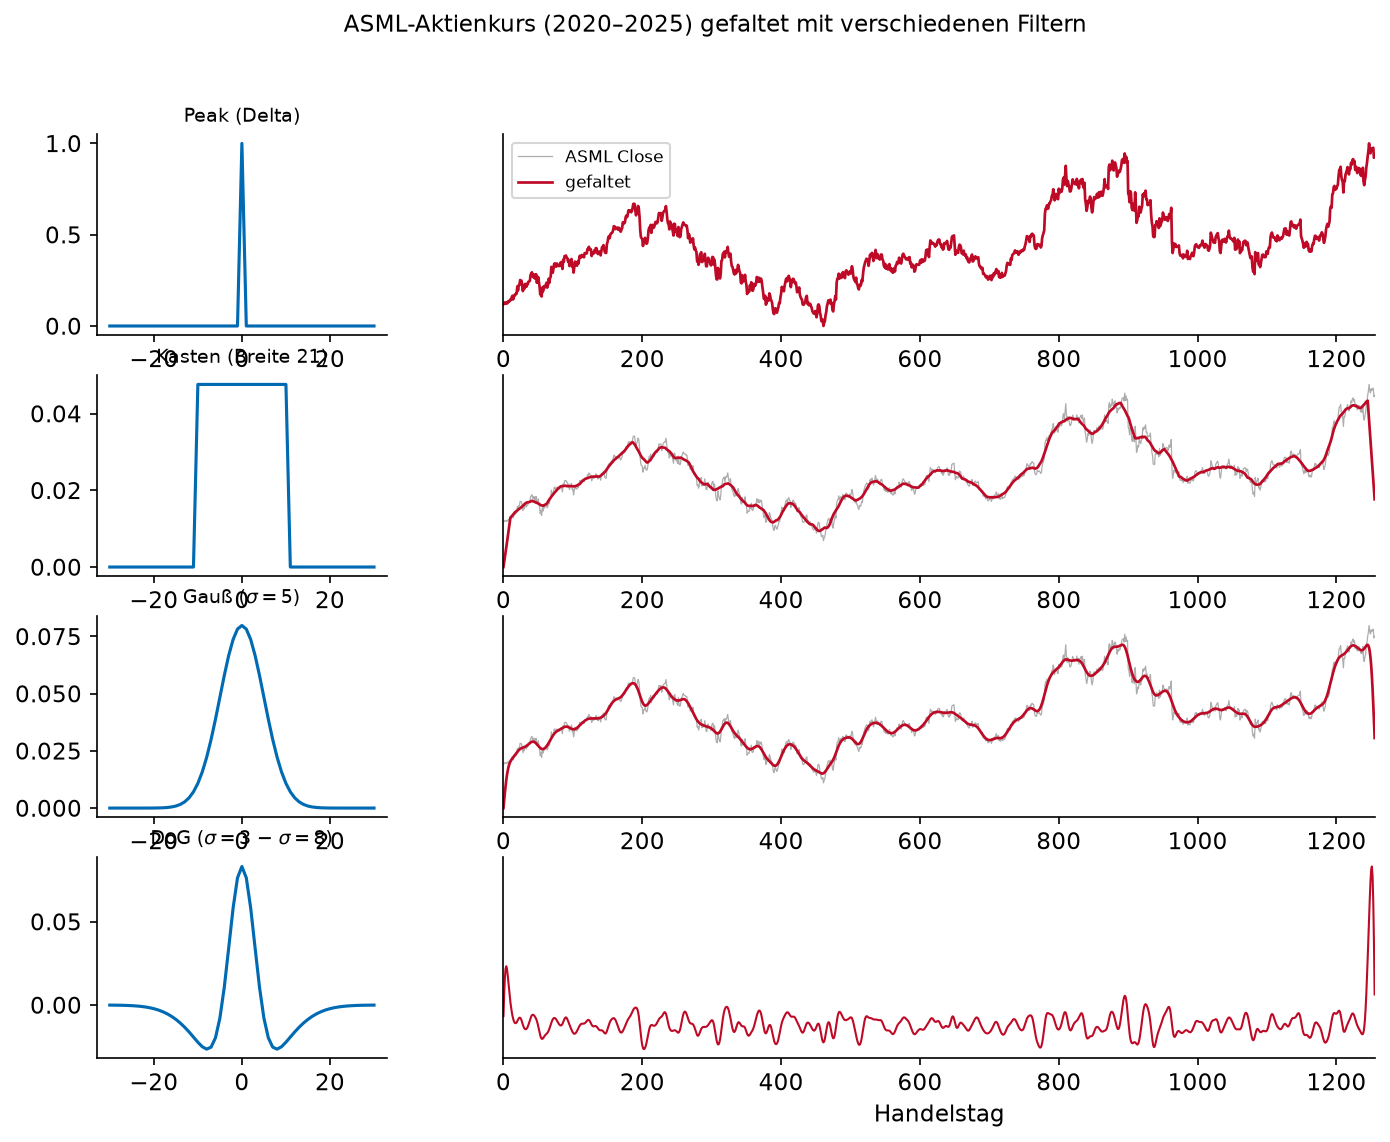
\includegraphics[height=0.62\textheight]{vl10-asml-convolutions.png}
  \end{center}

  \note{ASML-Schlusskurse 2020--2025. Delta lässt das Signal unverändert, Kasten und Gauß
    glätten (gleitender Mittelwert), die Difference of Gaussians hebt Änderungen hervor
    --- das ist ein Kantendetektor in 1D.
    Wer mag, kann hier schon fragen: Was wäre der Filter, der Kanten in einem Bild findet?}
\end{frame}

\begin{frame}
  \frametitle{Pooling}

  \begin{center}
    \Large
    Binning: disjunkte Blöcke\\[10pt]
    Pooling: Blöcke mit Überlapp, gesteuert vom \emph{Stride}\\[14pt]
    \normalsize Average-Pooling, Max-Pooling
  \end{center}

  \note{Pooling ist Dimensionsreduktion \emph{ohne Parameter} --- stumpfes Downsampling.
    Max-Pooling macht das Netz ein Stück weit translationsinvariant: Es ist egal, wo genau
    im Pool das Maximum lag.
    Alternativ kann man den Stride direkt in der Faltung verwenden (strided convolution),
    dann reduziert die Faltung selbst.}
\end{frame}

\begin{frame}
  \frametitle{Pooling, konkret}

  \begin{center}
    \Large
    $(a,b,c,d)$, Poolgröße 2, Stride 2\\[10pt]
    $\longrightarrow [\operatorname{mean}(a,b), \operatorname{mean}(c,d)]$\\[16pt]
    Poolgröße 3, Stride 1\\[10pt]
    $\longrightarrow [\max(a,b,c), \max(b,c,d)]$
  \end{center}

  \note{An der Tafel oder im Dialog durchspielen --- aus vier Werten werden zwei oder drei,
    je nach Größe und Stride. Mehr ist an Pooling wirklich nicht dran.}
\end{frame}

\begin{frame}
  \frametitle{Zweidimensional}

  \begin{center}
    \Large
    $(f \ast g)(x_1,x_2) = \sum_{y_1}\sum_{y_2} f(y_1,y_2)\,g(x_1-y_1, x_2-y_2)$
  \end{center}

  \bigskip
  \begin{center}
    \normalsize Ein $3\times3$-Filter: 9 Gewichte, an jeder Pixelposition dasselbe.
  \end{center}

  \note{Hier lohnt eine kleine Tafelskizze: das Filterfenster über dem Bild, das an jeder
    Position dasselbe Skalarprodukt bildet.
    Und dann GIMP: Filter $\to$ Allgemein $\to$ Faltungsmatrix --- dort trägt man die
    neun Werte selbst ein und sieht das Ergebnis sofort.}
\end{frame}

\begin{frame}
  \frametitle{Vier Faltungsmatrizen}

  \begin{center}
    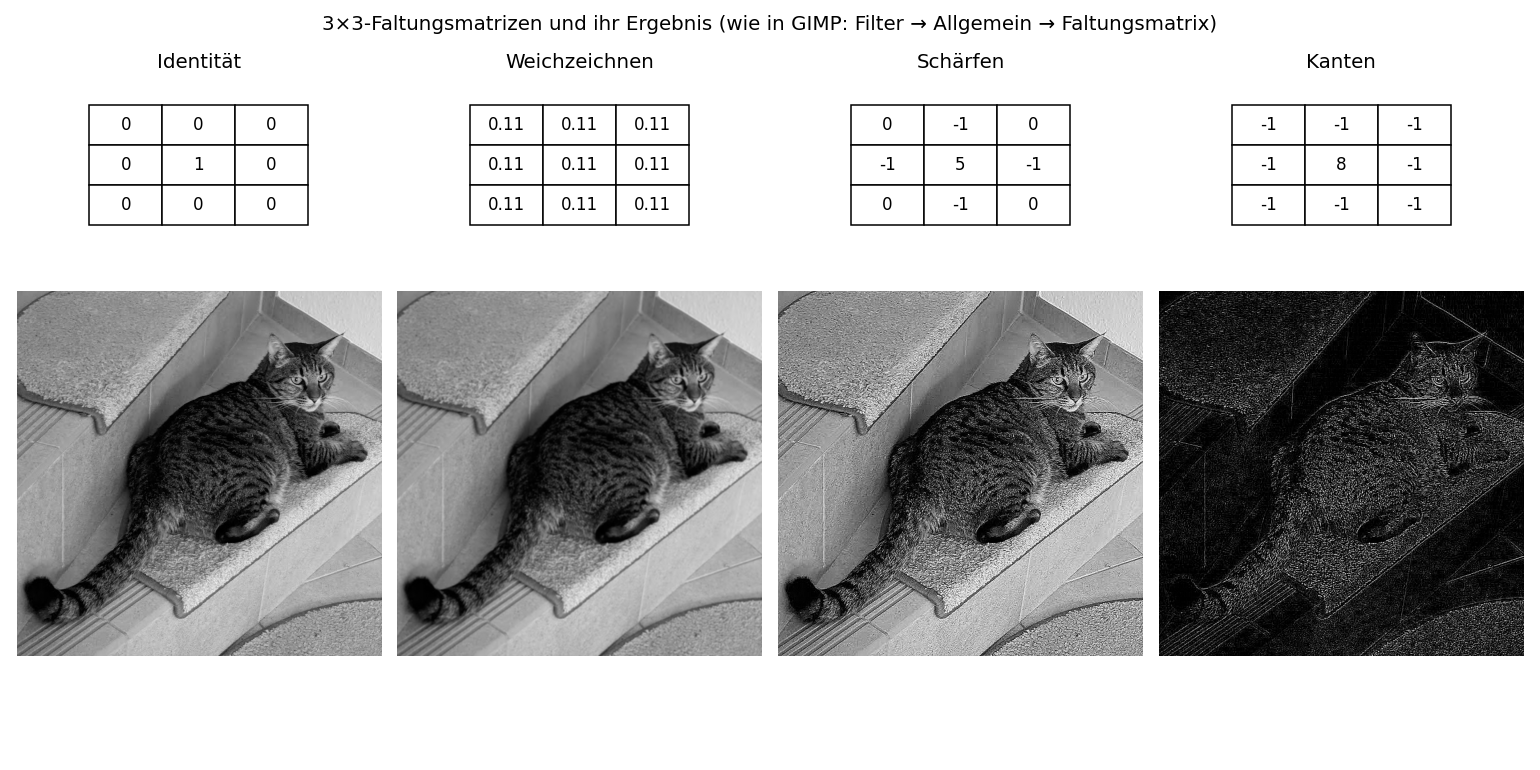
\includegraphics[width=0.66\textwidth]{vl10-faltungsmatrix.png}
  \end{center}

  \note{Identität, Weichzeichnen (Mittelwert), Schärfen, Kanten --- dieselben vier, die
    man in GIMP eintippen kann.
    Frage in den Raum: Welche neun Zahlen stehen wohl im Kanten-Filter? Die Antwort
    (Mitte positiv, Rand negativ, Summe null) kann man gemeinsam finden.}
\end{frame}

\begin{frame}
  \frametitle{Kanäle}

  \begin{center}
    \Large
    RGB-Bild: 3 Eingabekanäle\\[10pt]
    Ein Filter hat dann Shape $3 \times 3 \times 3$\\[10pt]
    $C_{\text{out}}$ Filter $\to$ $C_{\text{out}}$ Feature Maps
  \end{center}

  \note{Der Filter summiert über alle Eingabekanäle --- das ist wichtig und wird oft
    falsch gedacht.
    Ein $1\times1$-Filter schaut nur auf einen Pixel, aber über alle Kanäle: eine lineare
    Umrechnung im Kanalraum.
    Hier den Rückbezug zu VL 3 machen: \texttt{(32, 3, 28, 28)} --- Batch, Kanäle, Höhe,
    Breite.}
\end{frame}

\begin{frame}
  \frametitle{Ein CNN}

  \begin{center}
    \Large
    Conv $\to$ ReLU $\to$ MaxPool \; (mehrfach)\\[10pt]
    dann Flatten und Linear
  \end{center}

  \bigskip
  \begin{center}
    \normalsize $28 \to 24 \to 12 \to 8 \to 4$, \quad $16 \cdot 4 \cdot 4 = 256$
  \end{center}

  \note{Die Zahl im \texttt{nn.Linear} muss man ausrechnen --- das ist der häufigste
    Shape-Fehler beim Bau eines CNN. Mit \texttt{kernel\_size=3} statt 5 wären es
    $28 \to 26 \to 13 \to 11 \to 5$, also $16 \cdot 5 \cdot 5$.
    Nachgerechnet: Das Netz aus dem Skript liefert für einen $1\times1\times28\times28$-Batch
    tatsächlich Shape $(1, 10)$.}
\end{frame}

\begin{frame}
  \frametitle{Notebook}

  \begin{center}
    \Large \texttt{VL\_10\_convolutions.ipynb}
  \end{center}

  \bigskip
  \begin{center}
    \normalsize Faltung auf dem Aktienkurs, 2D-Filter auf einem Foto.
  \end{center}

  \note{\textbf{Etwa 20 Minuten, zeigen statt vorlesen.} Höhepunkt ist die Live-Änderung
    am 2D-Filter: die neun Zahlen ändern und sofort sehen, was mit dem Bild passiert.
    Wenn Zeit bleibt: conv\_arithmetic im Browser (animierte Faltungen mit Stride und
    Padding) und Harleys MNIST-CNN-Visualisierung.}
\end{frame}

\begin{frame}
  \frametitle{Bis nächste Woche}

  \begin{center}
    \Large Nächste Woche: Autograd --- und LLMs praktisch benutzen.
  \end{center}

  \note{Das nächste Übungsblatt (LLMs benutzen) kommt nächste Woche raus; das laufende Blatt
    (Faltung) ist nächsten Mittwoch fällig.
    Take-Home: Eine Faltung ist an jeder Stelle nur ein Skalarprodukt mit einem
    Ausschnitt, also billig; Pooling ist stumpfes Downsampling ohne Parameter. Und weil
    die Filter gelernt werden, kommen in den ersten Schichten von selbst dieselben
    Kantendetektoren heraus wie im Auge.}
\end{frame}

\end{document}

%%% Local Variables:
%%% mode: latex
%%% TeX-master: t
%%% End:
